\documentclass[9pt,twocolumn,twoside]{styles/osajnl}
\usepackage{fancyvrb}
\journal{i524} 
\usepackage[nomarkers,figuresonly]{endfloat}

\title{\centering%
Nagios (Example Paper for I524)}


\author[1]{Tony Liu}
\author[1]{Vibhatha Abeykoon}
\author[1]{Gregor von Laszewski}


\affil[1]{School of Informatics and Computing, Bloomington, IN 47408, U.S.A.}


\dates{paper-1, \today}

\ociscodes{Cloud, I524}

% replace this with your url in github/gitlab
\doi{\url{https://github.com/vibhatha/sp17-i524/blob/master/paper1/S17-TS-0003/report.pdf}}


\begin{abstract} Nagios is a system, network and infrastructure
  monitoring tool providing instant awareness of IT infrastructure.
  Nagios allows to monitor the infrastructure, alert the system admin,
  provide visualized reports, schedule downtime for maintenance, and
  plan upgrade in advance with trends and capacity diagrams. The
  design emphasizes highly on flexibility and scalability. We
  summarize details of Nagios and outline how it is useful as part
  ofthe services used in big data. \end{abstract}

\setboolean{displaycopyright}{true}

\begin{document}

\maketitle

\section{Introduction to Nagios}

Nagios ~\cite{www-nagios, wiki-nagios} is a system, network and
infrastructure monitoring tool under open source license that provides
instant awareness of mission-critical IT infrastructure. Nagios allows
to monitor the infrastructure, alert the system admin, provide
visualized reports, schedule downtime for maintenance, and plan
upgrade in advance with trends and capacity diagrams. Its design
emphasizes highly on flexibility and scalability. To provide such
flexibility, Nagios is composed of different modules. Through its
modular design Nagios cab adapt easily to systems and networks
monitoring needs by different users. It also allows integration of new
components that allow adaptation towards service monitoring needs that
have not yet been distributed with Nagios allowing extensibility.

\subsection{Architecture}

Nagios \cite{nagios-paper-2012} flexible modular architecture allows
users to customize modules to monitor the network and
infrastructure. We show the elementary Nagios archirtecture in
Figure~\ref{fig:Nagios-architecture} ~\cite{nagios-book}.

\begin{figure}[htbp]
\centering
\fbox{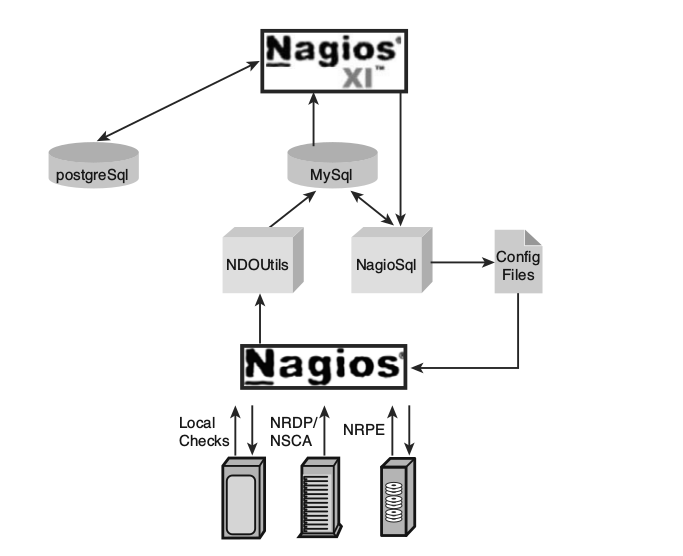
\includegraphics[width=\linewidth]{images/nagios-architecture}}
\caption{Nagios Architecture~\cite{nagios-book}.}
\label{fig:Nagios-architecture}
\end{figure}

<NOW DECSRIBE IT. THE IMAGE IS NOT THAT HELPFUL AS YOU DO NOT EXPLAIN
WHAT YOU SEE IN THE FIGURE>


Nagios has a number of components (a) ... (b) ... ....

The main component is {\em Nagios core}, which is a scheduler daemon
detecting network devices and services regularly. The core can alert
the administer through various notification methods like email,
message and web interface about system and event changes to alert of
issues and system states. Nagios plugin featues allows to register
events that can be triggered to execute actions actions and print
status updates.

I GOT TILL HERE GREGOR I HAVE TO WORK ON OTHER THINGS

It has two types,
check and notification. Both are used by Nagios core. The check plugin
is used to check and monitor devices and services. The notification
plugin is used to send out alerts if the check plugin detected any
status change. Beside these two, the users themselves can develop
their own custom plugins.

Nagios module is a procedure that calls upon API called Nagios Event
Broker. The user can develop the module with certain functionality and
embed within Nagios core. Whenever certain event triggers the module,
the module will be called to execute. The benefit of Nagios module is
that the user can access all necessary information within the core
process such as the Nagios status and check results.

Nagios' configuration file is text-based. It can be quite
sophisticated if the user wants to monitor large infrastructure. Also,
the user must understand the configurable options. Furthermore, since
it's text-based, the configuration file can be edited with a normal
editor. This can cause more trouble since there is no spellchecking or
proofreading. Luckily, there are tools helping users to generate
configuration files by applying configuration template with a
user-friendly web interface.

The last component is the web interface of Nagios. It's developed by
CGI technology in C programming language. This means compilation needs
every time new features and functionalities are added orderly. It is
not compatible with current popular web technologies like CSS, AJAX
and JQuery.

\section{Importance of Nagios}

Now it is clear the nature of Nagios and it's capabilities. There are
many reasons that has to be clarified, before deciding whether Nagios
is a vital tool to be used or not. Basically Nagios is a scalable and
a flexible solution for an organization. Due to the scalability, when
the structural changes or any changes happen, it is easier to fit the
new tools with Nagios, in order to manage them and monitor them. The
importance of Nagios can be explained through the different features
and facilities included.

\subsection{Comprehensive Monitoring}

Using Nagios there are many structures that can be monitored, and they
are operating systems, networking protocols, system metrics and
infrastructure components. And also there are many APIs to handle the
easy monitoring of in-house applications, services and systems. In
considering the network monitoring, basic use is the pinging and
Nagios uses it in a complex way and configurations are complex as it
is used to monitor many of the networking infrastructures. The feature
is post query support is also there in Nagios, this is very important
to monitor TCP or UDP connections with a particular host. The
capability of pinging and keeping track on multiple ports is also
enabled in this framework, so it is very easy to monitor a huge
network in a particular organization. And also when it comes to
service management, there are group service configurations that can be
added to the system by Nagios, this provides a variety of options to a
team to manage systems in a flexible way. There are a variety of
centralized views provided. For instance General view provides a
central dashboard which holds the keys to all other kinds of services
and tools like monitoring performance, network outage, etc. And also,
service details view provides the last check details, service type,
host and many other information related to services. This is a vital
tool, when it comes to managing thousands of services from a single
organization. Host details and host groups can also be viewed by the
tools in Nagios, this is very important to provide a more structured
service when an organization have a number of clients, so the group
management is a vital task when it comes to isolating services in
cases of maintenance and development. Collapsed tree status map and
marked up circular status map shows the connection between different
hosts and routers in a network. This is an important tool to identify
the service distribution and to identify breakdowns. By these views,
the failures can be notified by a physical and geographical location,
and this is a vital factor for a system management with less downtime.

\subsection{Problem Remediation}

In systems, there can be unexpected and expected problems when they
are running in live environments, so it is important to keep track on
these changes. Nagios provide alerting to such conditions. In case of
dealing with a fast recovery, there are automatic tools to recover the
failed components in a short time. These tools are very important in
case of providing services with less downtime.

\subsection{Visibility and Awareness}

The main feature expected from a tool is real time updates, reports
and status updates. In Nagios, the central dashboard provides these
facilities. As a tool, the most powerful thing is to share the
information in a centralized way, because there are many
administrative personnels dealing with data, in order to make
decisions.

\subsection{Reporting}

In referring to records and statistics, Nagios provide reporting tools
in order to keep track on the outputs from the dashboards and central
data collection systems, so that the data can be analyzed at the
present moment and also the ability to check the data in the history.
And also when it comes to tools like crystal reporting, casper
reporting, etc, Nagios provide support to third party tools so the
users can use the familiar reporting tools.

\subsection{Open-Source}

Nagios is an open source tool. MENTION LICENSE

\subsection{Multi-Tenant Capabilities}

In referring to a system, centralized access and multiple user login
to a system in a concurrent manner is very important. As mentioned
earlier, the dashboard in Nagios has the capability of providing
support to multiple users using the web interfaces. And the advantage
is that due to a web application, the installation is quite easy. The
web apps can be accessed through the network and the desktop
installation is not required, and the maintenance is also easier.

In referring to these factors, it is clear how Nagios can be used to
implement a solid foundation to maintain the information technology
based systems in an organization.

\section{Nagios for Big Data Application}

WRITE HOW NAGIOS CAN HELP BIG DATA APPLICATIONS

\section{Conclusion}

In referring to the architecture of Nagios, it is a very scalable and
flexible design. As a tool Nagios provide a wide variety of features
like system monitoring, alerting, maintenance, central administration,
etc. For an organization the most important thing is to keep track on
most of the tools and infrastructures they have. As far as the
organization grows, the most important factor is the scalable
monitoring capability with flexibility. And also the centralized
system administration is also another important feature expected by
most of the system administrators. Analyzing data is a vital factor in
taking management base decisions, for instance predicting costs for a
product, predicting system downtime, failures, etc can be done by
analyzing data. And also for a highly scaled organization, the number
of users and number of administrators that it has to handle grows by
every year, so the most important thing is to have an easy access to
the monitoring and managing tools. Nowadays, the attention paid to
desktop application is less, and more attention is paid to the web
applications. And also the multi-tenancy is also a vital factor when
it comes to manage many users at one time in order to provide customer
service to thousands or millions of users who consume a single
product. For a long term system management tool, the most important
fact is the continuous support, Nagios is a tool providing all these
requirement. In referring to all these facts, it is clear that for a
high end business solution provider, Nagios is a powerful tool to
support many tasks as mentioned.


% Bibliography

\bibliography{references}
 
%\newpage


\end{document}
